\chapter{Presentación del problema}

\section{Contexto y motivación}
La Escuela Superior de Medicina del Instituto Politécnico Nacional tiene su antecedente en la Carrera de Medicina Rural creada en 1938, desde entonces ha tenido varias adaptaciones y recintos, siendo el año de 1945 en el que fue creada por decreto oficial la Escuela Superior de Medicina Rural y finalmente en 1957 tuvo sus instalaciones propias, ya que en años previos había tenido que operar en instalaciones de otras Unidades Académicas del Instituto. En 1965 fue suprimido de su nombre el calificativo Rural y en lo sucesivo fue su nombre tal como actualmente se le conoce Escuela Superior de Medicina (ESM) y que es la Unidad Académica del IPN encargada de formar médicos cirujanos. (Fuente de referencia https://www.esm.ipn.mx/conocenos/mision.html)\\
Para cualquier estudiante de Medicina es fundamental y requisito conocer e interactuar con los sistemas del cuerpo humano, por ejemplo,  para la enseñanza de la anatomía y de morfología es indispensable el uso de cuerpos para su disección y análisis.\\
Actualmente en la Escuela Superior de Medicina y Homeopatía y la Escuela Superior de Medicina, utilizan principalmente medios impresos tradicionales y uso de cuerpos como principales materiales y recursos para  la enseñanza y aprendizaje.\\
El uso de cuerpos para su disección en la ESM tiene sus particularidades, por ejemplo, los costos inherentes al mantenimiento de los cuerpos en las instalaciones, frecuentemente se enfrenta el problema de que los cuerpos no son suficientes para la cantidad de alumnos en determinadas clases, algunas veces se deben de compartir los cuerpos con otras instituciones y cuando el cuerpo ya no puede seguir siendo utilizado se debe realizar su inhumación.\\
Hay además algunas problemáticas que ha enfrentado la ESM, como el mantenimiento óptimo de las instalaciones, particularmente relacionado a lo que se ha mencionado del uso de los cuerpos para exploración, del anfiteatro. Sobre esto a raíz del sismo de septiembre de 2017, se dañaron varios edificios así como el anfiteatro, en el caso de este último quedando inutilizable durante casi seis meses, lo cual obligó  a los docentes a reformular sus clases de morfología y anatomía usando presentaciones de diapositivas y algunos videos. Este tipo de problemas incide directamente en la parte práctica que debe realizar el estudiante de medicina, en este caso en particular, en el semestre siguiente el rendimiento de los estudiantes se vio disminuido a causa de la falta de práctica física con los cuerpos.\\
Teniendo conocimiento de este tipo de problemas y con la intención de crear una herramienta de software que utilizará la Realidad Virtual, en septiembre de 2018 se entrevistó al Dr. Rios Macias Jefe del Área de Morfología de la Escuela Superior de Medicina (ESM) del Instituto Politécnico Nacional (IPN) y comentó que “los medios que se utilizan para el estudio del cuerpo humano principalmente son impresos tradicionales, así como el uso de cuerpos para su disección y análisis posterior”. Derivado de las entrevistas realizadas, se sabe que, son muchos los subsistemas del cuerpo humano y que la creación de materiales distintos a los libros y materiales impresos, puede ser un área de oportunidad que ofrezca a los estudiantes una alternativa extra para explorar y reforzar sus conocimientos, aunque hasta ahora no es posible reemplazar la interacción de los estudiantes con el cuerpo humano real.1.2 Propuesta de Solución
Considerando que son muchos los subsistemas que integran el cuerpo humano, se ha elegido el sistema digestivo. Por lo tanto, este documento presenta un prototipo de sistema de realidad virtual del sistema digestivo del cuerpo humano que permite interactuar con modelos tridimensionales de los órganos que lo conforman. La intención podría ser sentar un precedente de un sistema de apoyo al aprendizaje que favorezca la interacción práctica [ 1 ] de los estudiantes de la ESM.\\

\section{Objetivos del Sistema}
Analizar, diseñar, desarrollar y probar un prototipo de sistema que utiliza la tecnología de Realidad Virtual, para ofrecer una experiencia orientada al estudio 
de la anatomía y morfología del cuerpo humano, específicamente del sistema digestivo.\\
\subsection{Objetivos Específicos}
\begin{itemize}
	\item Utilizar como insumo para la elaboración de los modelos, las referencias documentales y confiables que proporcionan los expertos del área de morfología de la ESM del IPN sobre el sistema digestivo.
	\item Elaboración de modelos en tres dimensiones del sistema digestivo humano
	\begin{enumerate}
		\item Glándulas Salivales
		\item Cavidad Oral
		\item Faringe
		\item Esófago
		\item Estómago
		\item Intestino Delgado
		\begin{enumerate}
		  \item Hígado
		  \item Páncreas
		  \item Vesícula Biliar
		\end{enumerate}
		\item Intestino Grueso y Ano  
	\end{enumerate}
	\item Diseñar y desarrollar
	\item Probar los componentes de software del sistema y realizar su interacción con los elementos de hardware que propiamente proporcionan el entorno de  Realidad Virtual.	
\end{itemize}

\section{Revisión del Estado del Arte}
A continuación se muestran algunos de trabajos académicos desarrollados en México y fueron comparados con el trabajo planeado. 
Como comparativa y de forma ilustrativa del sector académico.\\
\newline
\begin{enumerate}
\item TT No. 2014-A058 “Sistema para la orientación de los efectos sobre la espalda humana en pacientes con sobrepeso”\cite{tt1}
\item TT No. 2012-B055 “Laboratorio Virtual del cuerpo humano 3D con asistente de ayuda en línea para el nivel superior bajo el paradigma de Educación Basada en Web con 
tecnologías de Web Semántica”\cite{tt2}
\item TT No. 2014-B035 “Simulación en Tercera Dimensión del Sistema Circulatorio de los Cánidos para el uso Educativo”\cite{tt3}
\item TT No. 2014-B039 “Simulación de una Línea del Metro con Realidad Virtual”\cite{tt4}
\item Tesis que para optar por el grado de Maestro en Ciencia e Ingeniería de la Computación, Sistema de seguimiento de movimiento de las extremidades superiores basado 
en sensores inerciales para rehabilitación en realidad virtual.\cite{mastersthesis1}
\item Adecuación educativa de la realidad virtual como herramienta didáctica para el proceso enseñanza-aprendizaje / tesis que para obtener el título de Licenciado en 
Pedagogía, presenta Maria de la O García Noriega; asesor Lucina Moreno Valle Suárez.\cite{te1}
\end{enumerate}
Así mismo se ha encontrado software propietario desarrollado por empresas privadas los cuales son los siguientes.\\
\begin{itemize}
\item The Body VR: Anatomy Viewer es la única herramienta de visualización de Realidad Virtual disponible en el mercado que se basa en datos médicos específicos del 
paciente (por ejemplo, MRI, CT, PET) y cumple con los estándares DICOM. Proporciona simulaciones de RV anatómicas en tiempo real para visualizar diagnósticos médicos, 
ilustrar el impacto de los procedimientos y tratamientos, y crear una toma de decisiones más educada.\
\begin{figure}[H]
	\begin{center}
 		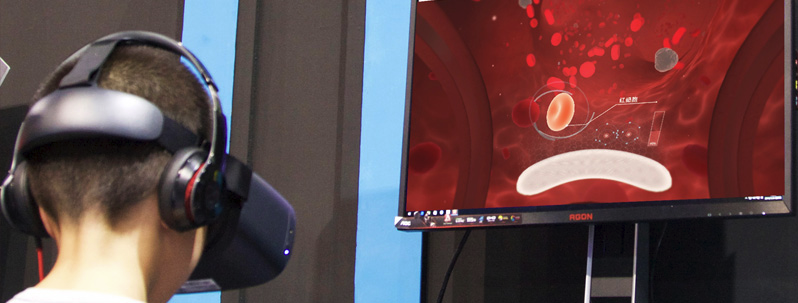
\includegraphics[width = 0.5\textwidth]{source/images/image9.png}
 		\captionof{figure}{\label{fig:ea1}Software “The Body VR” en uso.}
	\end{center} 
\end{figure}
\item Anatomyou VR: Estructuras anatómicas fotorrealistas, modeladas en colaboración con RenderArea, validadas por expertos clínicos y certificadas por personal capacitado 
en  Tecnologías Médicas de la Universidad de Las Palmas de Gran Canaria.
\begin{figure}[H]
	\begin{center}
 		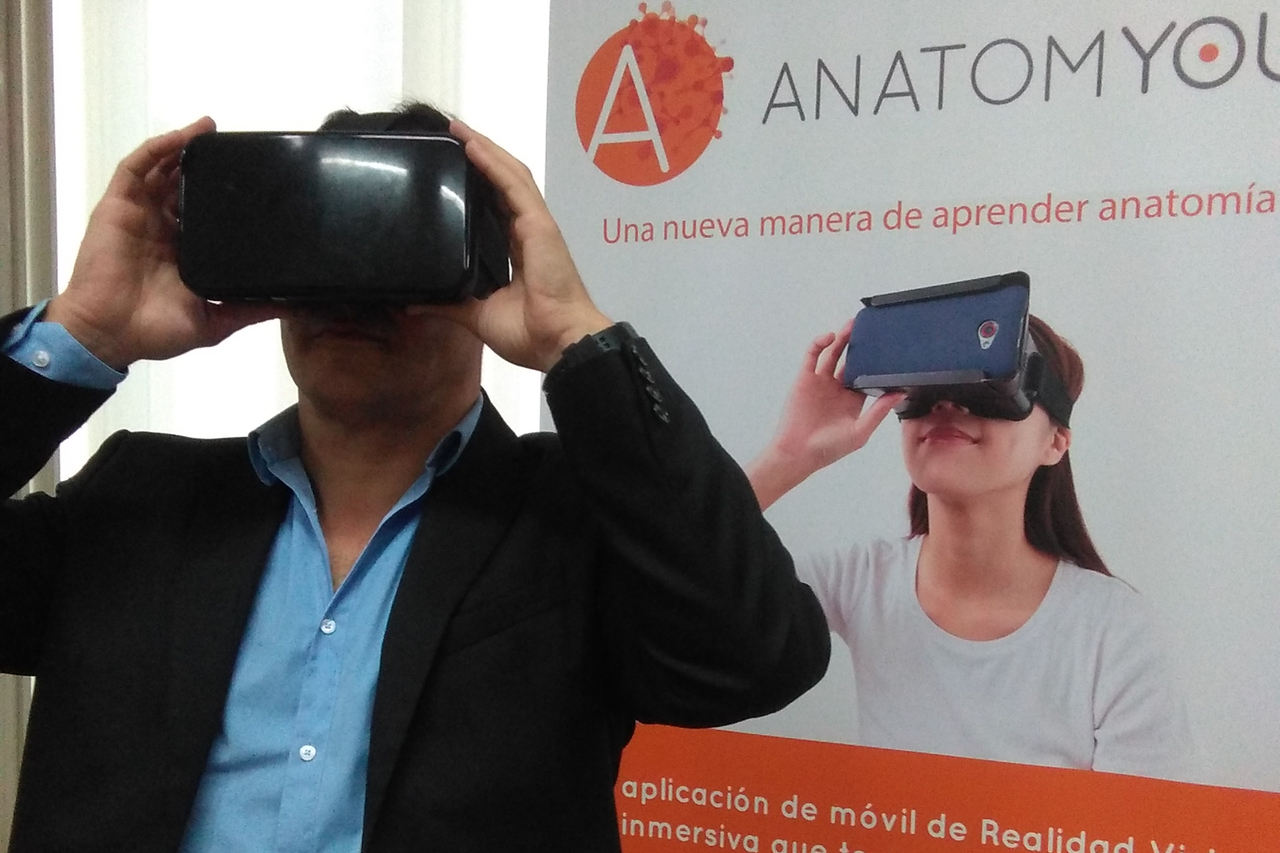
\includegraphics[width = 0.5\textwidth]{source/images/image59.png}
 		\captionof{figure}{\label{fig:ea2}Pancarta promocional de “Anatomyou VR}
	\end{center} 
\end{figure}
\item Biodigital Anatomy: El cuerpo tridimensional más completo, científicamente preciso e interactivo jamás ensamblado. Anatomía masculina y femenina, en los detalles 
básicos (gratuitos) y profesionales. Cada sistema está completamente segmentado, etiquetado y direccionable para una fácil configuración que satisfaga cualquier necesidad educativa.
\begin{figure}[H]
	\begin{center}
 		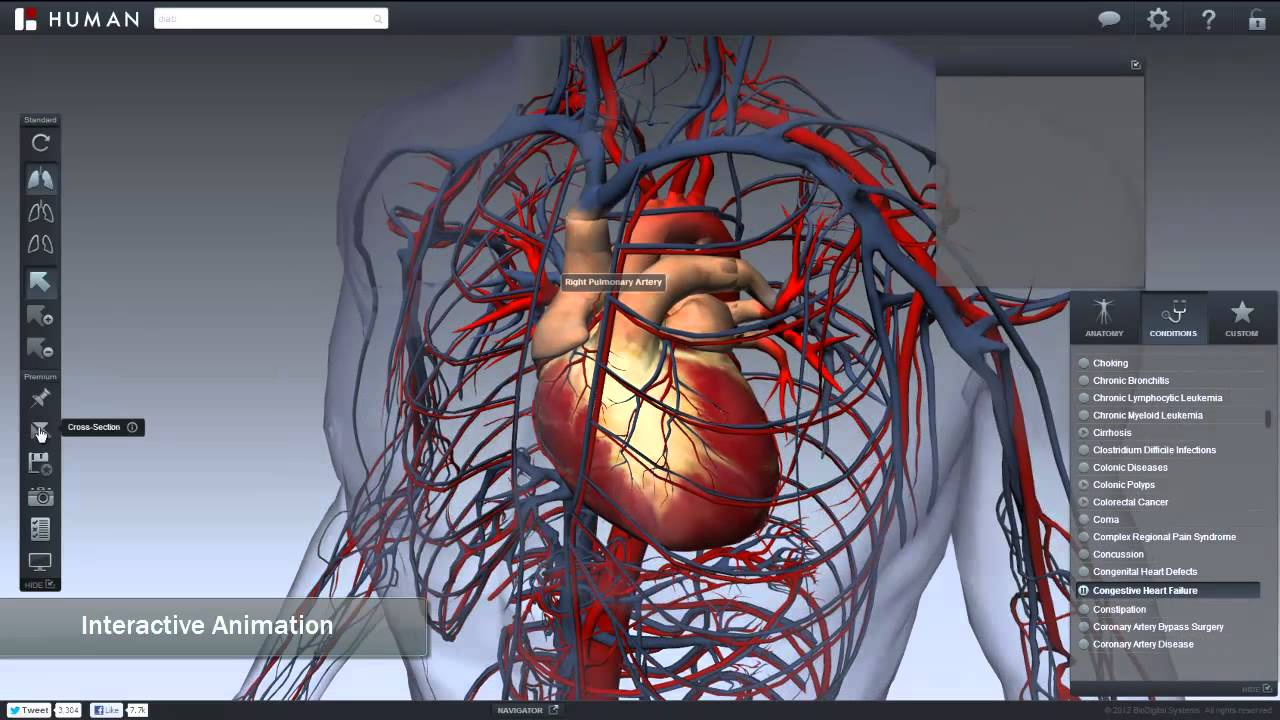
\includegraphics[width = 0.5\textwidth]{source/images/image18.png}
 		\captionof{figure}{\label{fig:ea3}Interfaz del software de Biodigital Anatomy}
	\end{center} 
\end{figure}
\item 3D Organon VR Anatom: 3D Organon es un completo atlas anatómico que presenta los 15 sistemas del cuerpo humano. Incluye más de 4,000 estructuras y órganos anatómicos 
realistas y más de 160 correlaciones clínicas encontradas por sistema del cuerpo.
\begin{figure}[H]
	\begin{center}
 		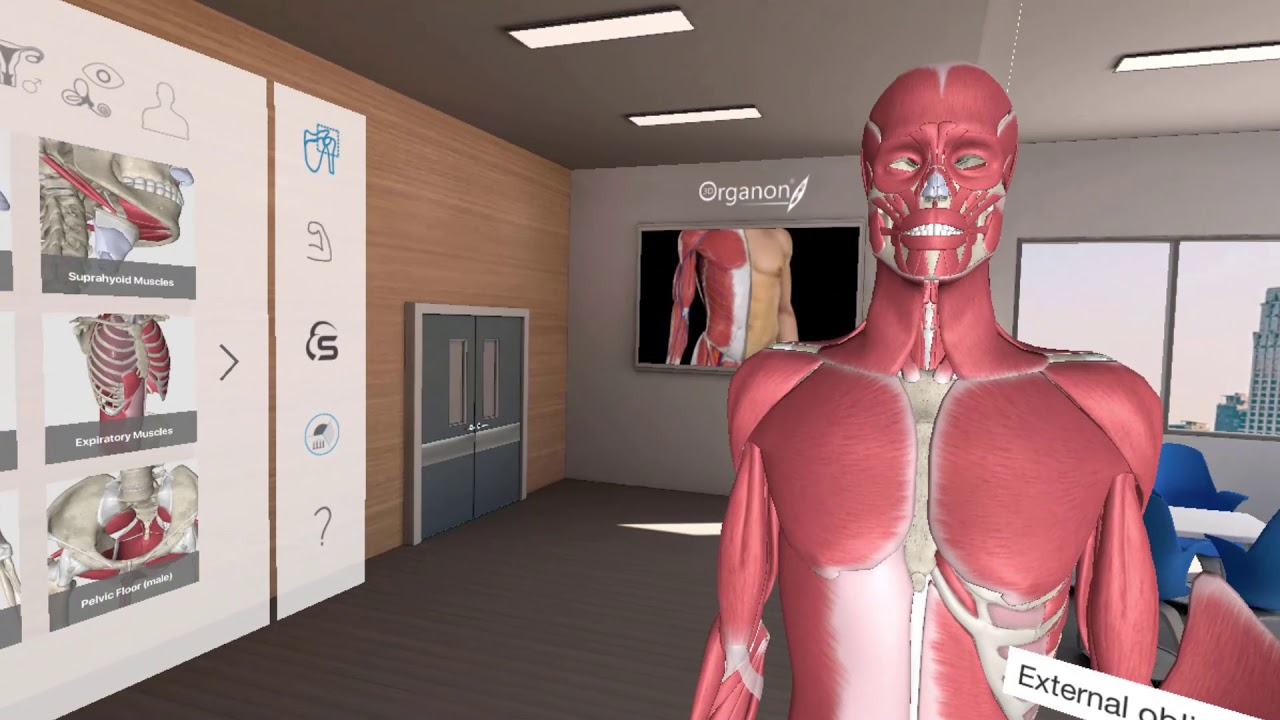
\includegraphics[width = 0.5\textwidth]{source/images/image5.png}
 		\captionof{figure}{\label{fig:ea4}Interfaz del software de 3D organon VR Anatom}
	\end{center} 
\end{figure}
\end{itemize}

\section{Organización de capítulos}
Este documento es el reporte técnico final del trabajo terminal titulado “Sistema de Realidad Virtual del Cuerpo Humano para el Estudio del Sistema Digestivo” con número de registro TT: 2019-A104.\\
En el \textbf{Capítulo} presente se habla del contexto y la motivación que dieron parte a la realización  de este, por qué se considera como tal y cómo es que se ayudó a resolver el problema planteado mediante la ingeniería en sistemas computacionales. También se menciona que se obtiene al concluir con este trabajo terminal, tales como el prototipo del sistema.\\
El \textbf{Capítulo II Marco Teórico} muestra conceptos que se consideran útiles para contextualizar este Trabajo Terminal. Presenta conceptos de ...%% TODO: inserta aquí las dos disciplinas que comentas.
En el \textbf{Capítulo III Soluci\'on Propuesta} se describe el trabajo generado en el desarrollo del documento hasta el mes de mayo de 2020 para TT2.\\
En el \textbf{Capítulo IV Pruebas Experimentales} se muestran pruebas hechas sobre las implementaciones del sistema siguiendo un guión para la prueba.\\ 
En el \textbf{Capítulo V Conclusiónes y Trabajo a Futuro} se encuentran las conlusiones sobre resultados obtenidos y experiencias para mejorar el proceso, así como la vertiente para continuar con el trabajo.\\
Finalmente, se encuentran las \textbf{Referencias} de todos los recursos empleados para dar soporte y estructura a este Trabajo Terminal, y en los apéndices se anexan elementos extra que dan información más detallada sobre lo que aquí fue realizado.\\
